
\section{Two Dimensional Analysis}
This section will discuss the trends and effect of various undertray variables in two dimensions. The variables tested consist of the inlet and diffuser angles, and the optimised values will be used as a preliminary variable for the three dimensional undertray design. The 2D analysis will consist of an enclosed flow analysis, which uses a Venturi-tube like geometry to simulate the undertray flow, and an open flow analysis, which uses a bluff body to simulate the flow behaviour, as well the interaction between the undertray and the bluff body. 

\subsection{2D Enclosed Flow}
The analysis of the 2D enclosed flow serves the purpose of building a fundamental understanding of undertray flow physics. The diffuser and inlet angles were chosen to be the main variables which are fundamentally known to affect the undertray's performance. It is described as 'Enclosed' due to its geometry being shaped like a half Venturi tube, which restricts the flow analysis to only the lower part of the undertray without any consideration of the surrounding flow ahead of and behind the car itself. 

\subsubsection{Geometry and Mesh Generation}
\noindent The general geometry is shown in Figure~\ref{fig:2D_EN_Geom} below. A realistic preliminary dimension was chosen to obtain a general picture of the undertray shape in 2D. The geometry represents the underside of the car, which consists of the undertray (top-wall), moving floor (bottom-wall), velocity inlet (left), and outlet (right). At this stage, the car's length was estimated to be 2000 mm, with 200 mm inlet and 600 mm diffuser horizontal length. Gap clearance (the minimum distance between the undertray and the floor) was chosen to be 30 mm, which complies with the minimum gap clearance distance rules of FSUK. Two sets of undertray geometries were generated by varying two variables. The first is generated by increasing the diffuser angle from 10 to 20 degrees in increments of two degrees, accompanied with an inlet angle of 10 degrees for every geometry. The second set is generated by increasing the inlet angle from 10 to 20 degrees in increments of two degrees, accompanied with a 10 degree diffuser angle for every geometry. This approach allows for a preliminary development in understanding the effect of both the undertray's outlet and inlet angle in an isolated flow-field. 

\begin{figure}[!ht]
    \centering
    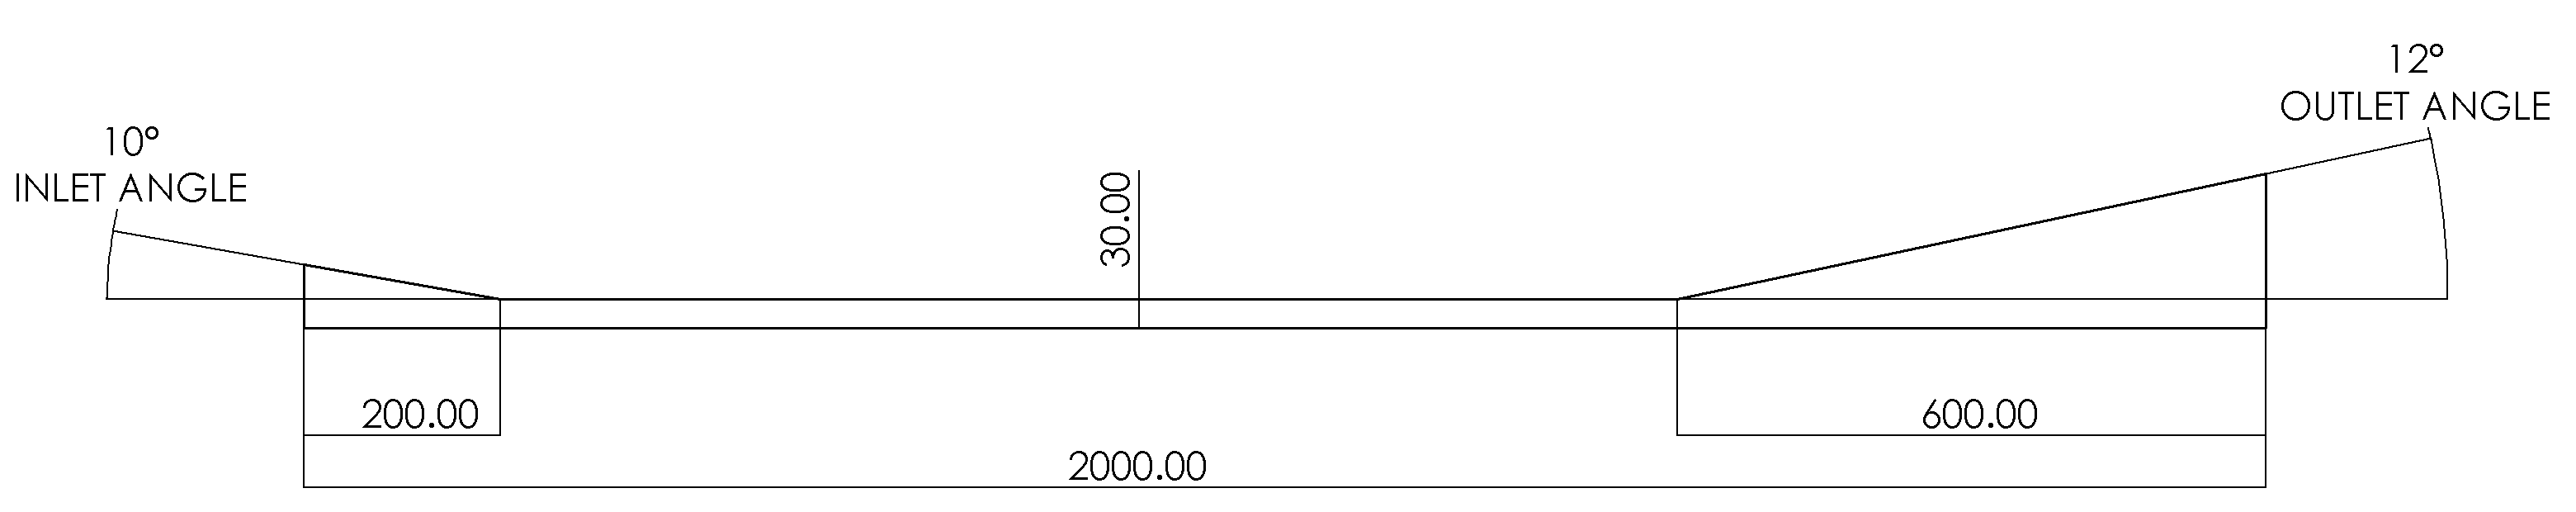
\includegraphics[scale=0.18]{Figures/2D_EN/2D_EN_D.PNG}
    \caption{2D Enclosed Geometry.}
    \label{fig:2D_EN_Geom}
\end{figure}
  
\noindent A structured quadrilateral mesh was generated, and the inflation layer was initialised on the underside of the undertray. Twenty layers of inflation were used with an initial value of $y^+ = 1$, which gives the first layer distance of $2.24 \times 10^{-5}$ meters. Generally, the number of mesh elements generated for each geometry in the 2D enclosed flow analysis was around 20000 to 25000, depending on the exact geometry. The resulting mesh quality was good, with a skewness average of $3.67 \times 10^{-2}$ and an aspect ratio average of $31$, which is slightly above the recommended range \cite{Lanfrit2005BestFLUENT}; however, the convergence criterion was still met. Figure~\ref{fig:2D_EN_MESH} in Appendix A shows a mesh generated from one of the 2D enclosed geometries, along with the details of the inflation layer.

\subsubsection{Results \& Discussion}
These simulations will be discussed based on how changes in outlet and inlet angle affected the downforce (negative lift) and drag of the undertray. Figure~\ref{fig:2D_EN_result} shows the lift and drag of the simulations for both geometry sets and both turbulence models. Figure~\ref{fig:2D_EN_result} shows the trend of undertray lift and drag with changing diffuser angle variable on the left, and with the inlet angle variable on the right. 

\noindent $k-\epsilon$ and $k-\omega$ turbulence models were employed in this analysis, as recommended\cite{} and discussed in section \ref{section: Numberical Method}. As shown in Figure~\ref{fig:2D_EN_result} below, a similar trend in performance emerged for both turbulence models. There was no significant difference found between the two numerical methods; however, some anomalies were found to occur in some of the results. For instance, both the $k-\omega$ lift at 16-degree diffuser and inlet angle, and the $k-\omega$ drag at 20-degree inlet angle are considered to be a little higher than the trend pattern. Nonetheless, the pattern emerging from both sets of geometries and turbulence models are clear, and can be used to give a preliminary understanding of the undertray flow physics.

\begin{figure}[!ht]
  \noindent
  \makebox[\textwidth]{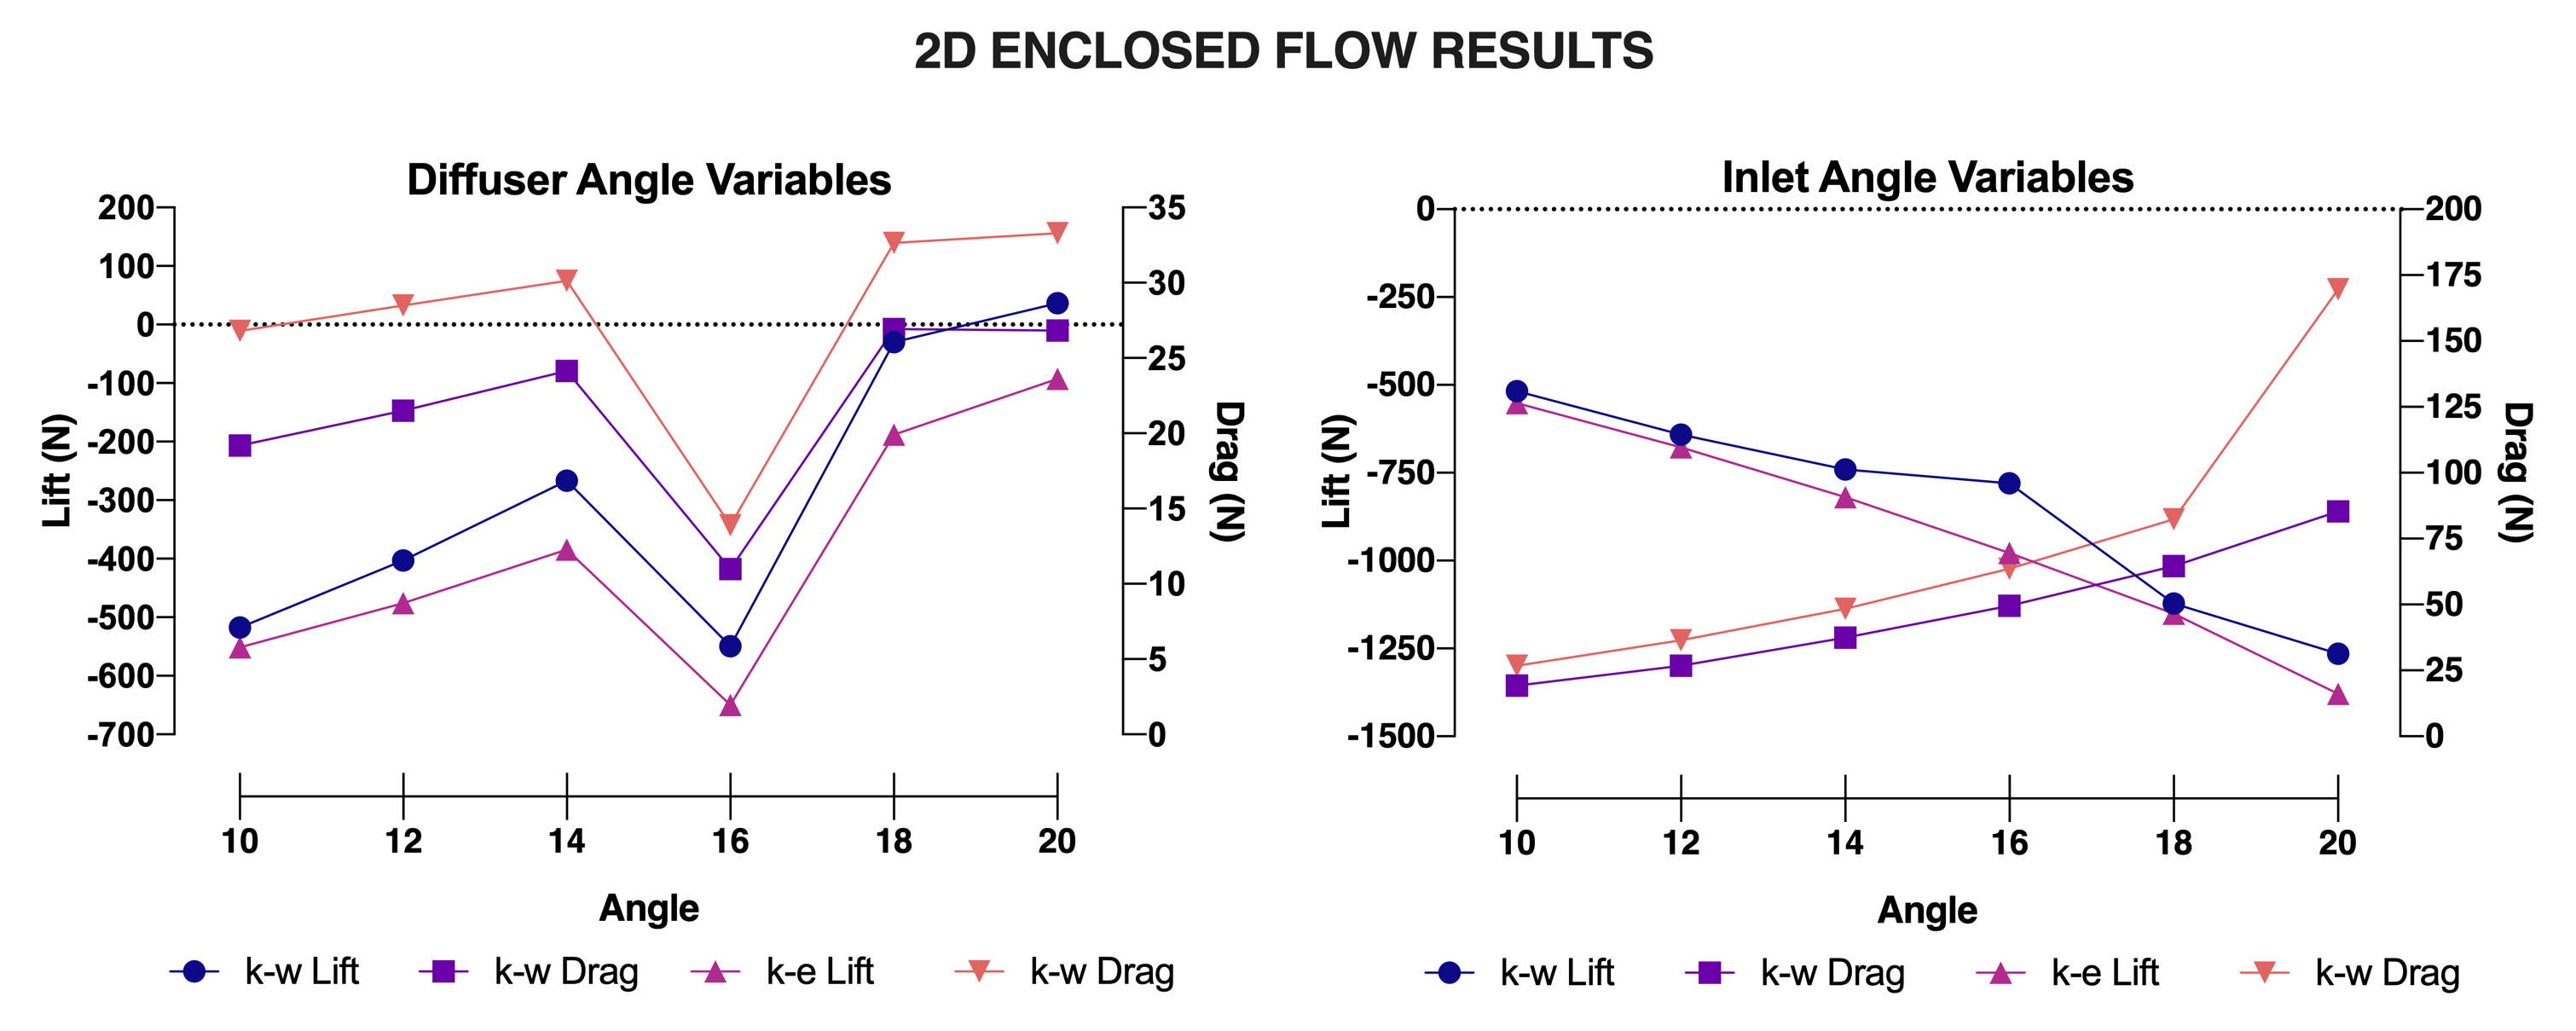
\includegraphics[scale=0.65]{Figures/Graph/2D_EN.png}}
  \caption{Lift and Drag Plot of 2D Enclosed Flow Analysis Trend for Both Diffuser (left) and Inlet (right) Angle Variables.}
  \label{fig:2D_EN_result}
\end{figure}

\noindent The main goal of a diffuser is to slowly expand the accelerated flow from the undertray's throat, acting as the pressure and flow recovery system of an undertray. An efficient diffuser allows gradual pressure recovery, which indicated by the flow remaining attached along the diffuser's wall. However, the diffuser angle variable plot on Figure~\ref{fig:2D_EN_result} (left) shows a linear degradation in the undertray's performance. This trend shows that an increase in diffuser angle is directly proportional to the undertray's lift and drag. This is generally due to early flow separation in the transition region between the undertray's throat and diffuser region. 

\noindent The sharp corner and high velocity are the main issues that cause the flow to detach early and create a sudden pressure change. Figure~\ref{fig:2D_EN_streamline_compare} shows the velocity streamline for both the 10 degree and 20 degree diffuser angles. The figure shows a similar separation point of the streamline in both cases when the flow enters the diffuser region. This phenomenon is more obvious for the larger diffuser angle (Figure~\ref{fig:2D_EN_streamline_compare} right) as a lower pressure region is formed, indicated by the dark blue colour. Linear increases in drag are explained by the low pressure region formed on the diffuser area, which acts as a vacuum that pulls the undertray contrary to its forward motion.  

\begin{figure}[!ht]
    \centering
    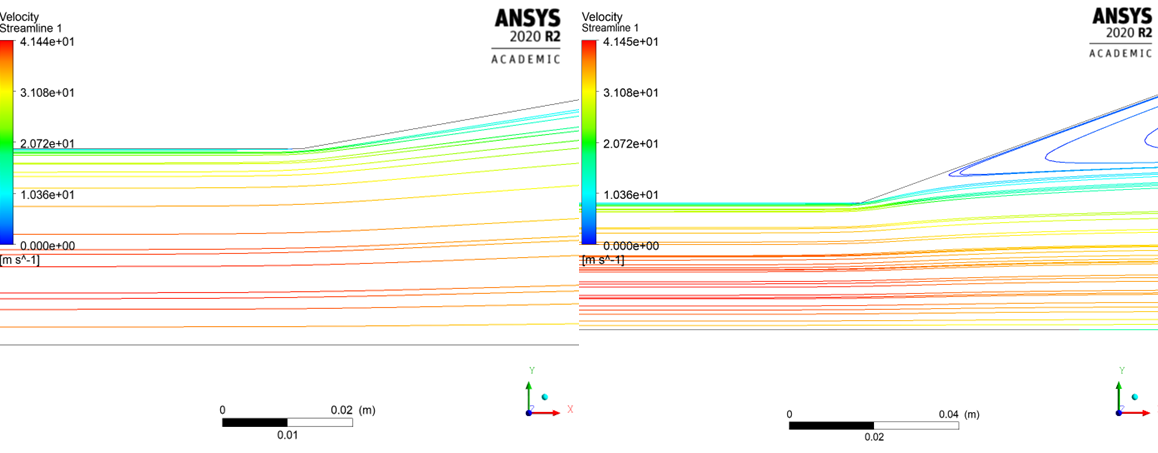
\includegraphics[height= 6cm]{Figures/2D_EN/2D_EN_Streamline_compare.PNG}
    \caption{Undertray Velocity Streamlines for 10 Degree (left) and 20 Degree (right) Diffuser Angles.}
    \label{fig:2D_EN_streamline_compare}
\end{figure}

\noindent From Figure~\ref{fig:wall_shear_plot_2D_EN} (left) in Appendix A, it can be observed that flow detachment occurs at an identical point on the undertray for any given diffuser angle, which is indicated by a similar pattern of the second peak on the graph. Moreover, the flow detachment occurs due to the sudden high adverse pressure gradient, which is indicated on the second lower peak on the static pressure plot in Figure~\ref{fig:pressure_plot_2D_EN} in Appendix A.

\noindent On the other hand, changing the inlet angle variable has an opposite effect to the previous variable. Figure~\ref{fig:2D_EN_result} (right) shows that the lift scales inversely to the drag as the inlet angle is increased. As the cross-sectional area reduces as the inlet nozzle converges, the flow is forced to convert the pressure energy into kinetic energy, indicated by the increase in its velocity, which then lowers the static pressure in the undertray's throat. This condition creates a lower pressure region on the undertray's throat, hence increasing the downforce. This phenomenon, in an ideal flow, obeys Bernoulli's equation (Equation~\ref{eq:bernoulli}), where pressure and cross-sectional area are inversely proportional to the flow's velocity, assuming the flow in the inlet region is steady and incompressible. There is also a geometric effect --- increasing the inlet angle provides more flow normal surface area for the pressure field to act over, creating higher normal forces on the inlet wall and increasing the overall drag. The wall shear force also increases, which is indicated on the first peak in the wall shear on Figure~\ref{fig:wall_shear_plot_2D_EN} (left), which shows a significant increase in shear stress at the corner between the inlet and throat region.

\noindent Further analysis of wall shear stress (Figure~\ref{fig:wall_shear_plot_2D_EN} right) and static pressure (Figure~\ref{fig:pressure_plot_2D_EN} right) plots for inlet angle variables in Appendix A show a general increase in shear stress with inlet angle, accompanied by the overall pressure drop as the angle increases. This explains the increase in total downforce with the increase of the inlet angle.

\noindent This analysis has a number of limitations. First, the flow only includes the underpart of the undertray, making these simulations geometrically ideal as the intake and outlet flow acceleration and deceleration are efficient. Without taking the surroundings of the flow into consideration, a linear trend could easily be achieved, as discussed. This analysis cannot, therefore, supply benchmark results for the undertray prototype design, however a broad understanding of the flow behaviour was obtained.

%%%%%%%%%%%%%%%%%%%%%%%%%%%%%
%%% 2D OPEN FLOW ANALYSIS %%%
%%%%%%%%%%%%%%%%%%%%%%%%%%%%%


\subsection{2D Open Flow}
The previous analysis provided a fundamental understanding of how changes in inlet and diffuser angle might affect undertray performance, and solely focused on the internal flow of the undertray without taking account of the flows around it. This section extends the previous analysis in order to better understand the effect of similar variable changes, but with an additional bluff body added to the geometry. 

\subsubsection{Geometry and Mesh Generation}
This section utilises multiple types of bluff body to simulate the flow behaviour and explore how this affects an undertray's general performance. Four different geometries were built, with each serving its own purpose. A rough calculation of the QFR car's length was required. Geometry 1 \& 2 have 2.6 meters of undertray length, with a similar inlet and diffuser configuration as in the previous analysis. However, Geometry 3 represents a slightly different undertray configuration, with 2.85 meters of length, a 1-meter smoothly rounded diffuser, and 0.25 meters of inlet. It is worth noting here that the code 'A' stands for 'analysis', which corresponds to the type of geometry used in the discussions and figures.

\begin{figure}[!ht]
    \centering
    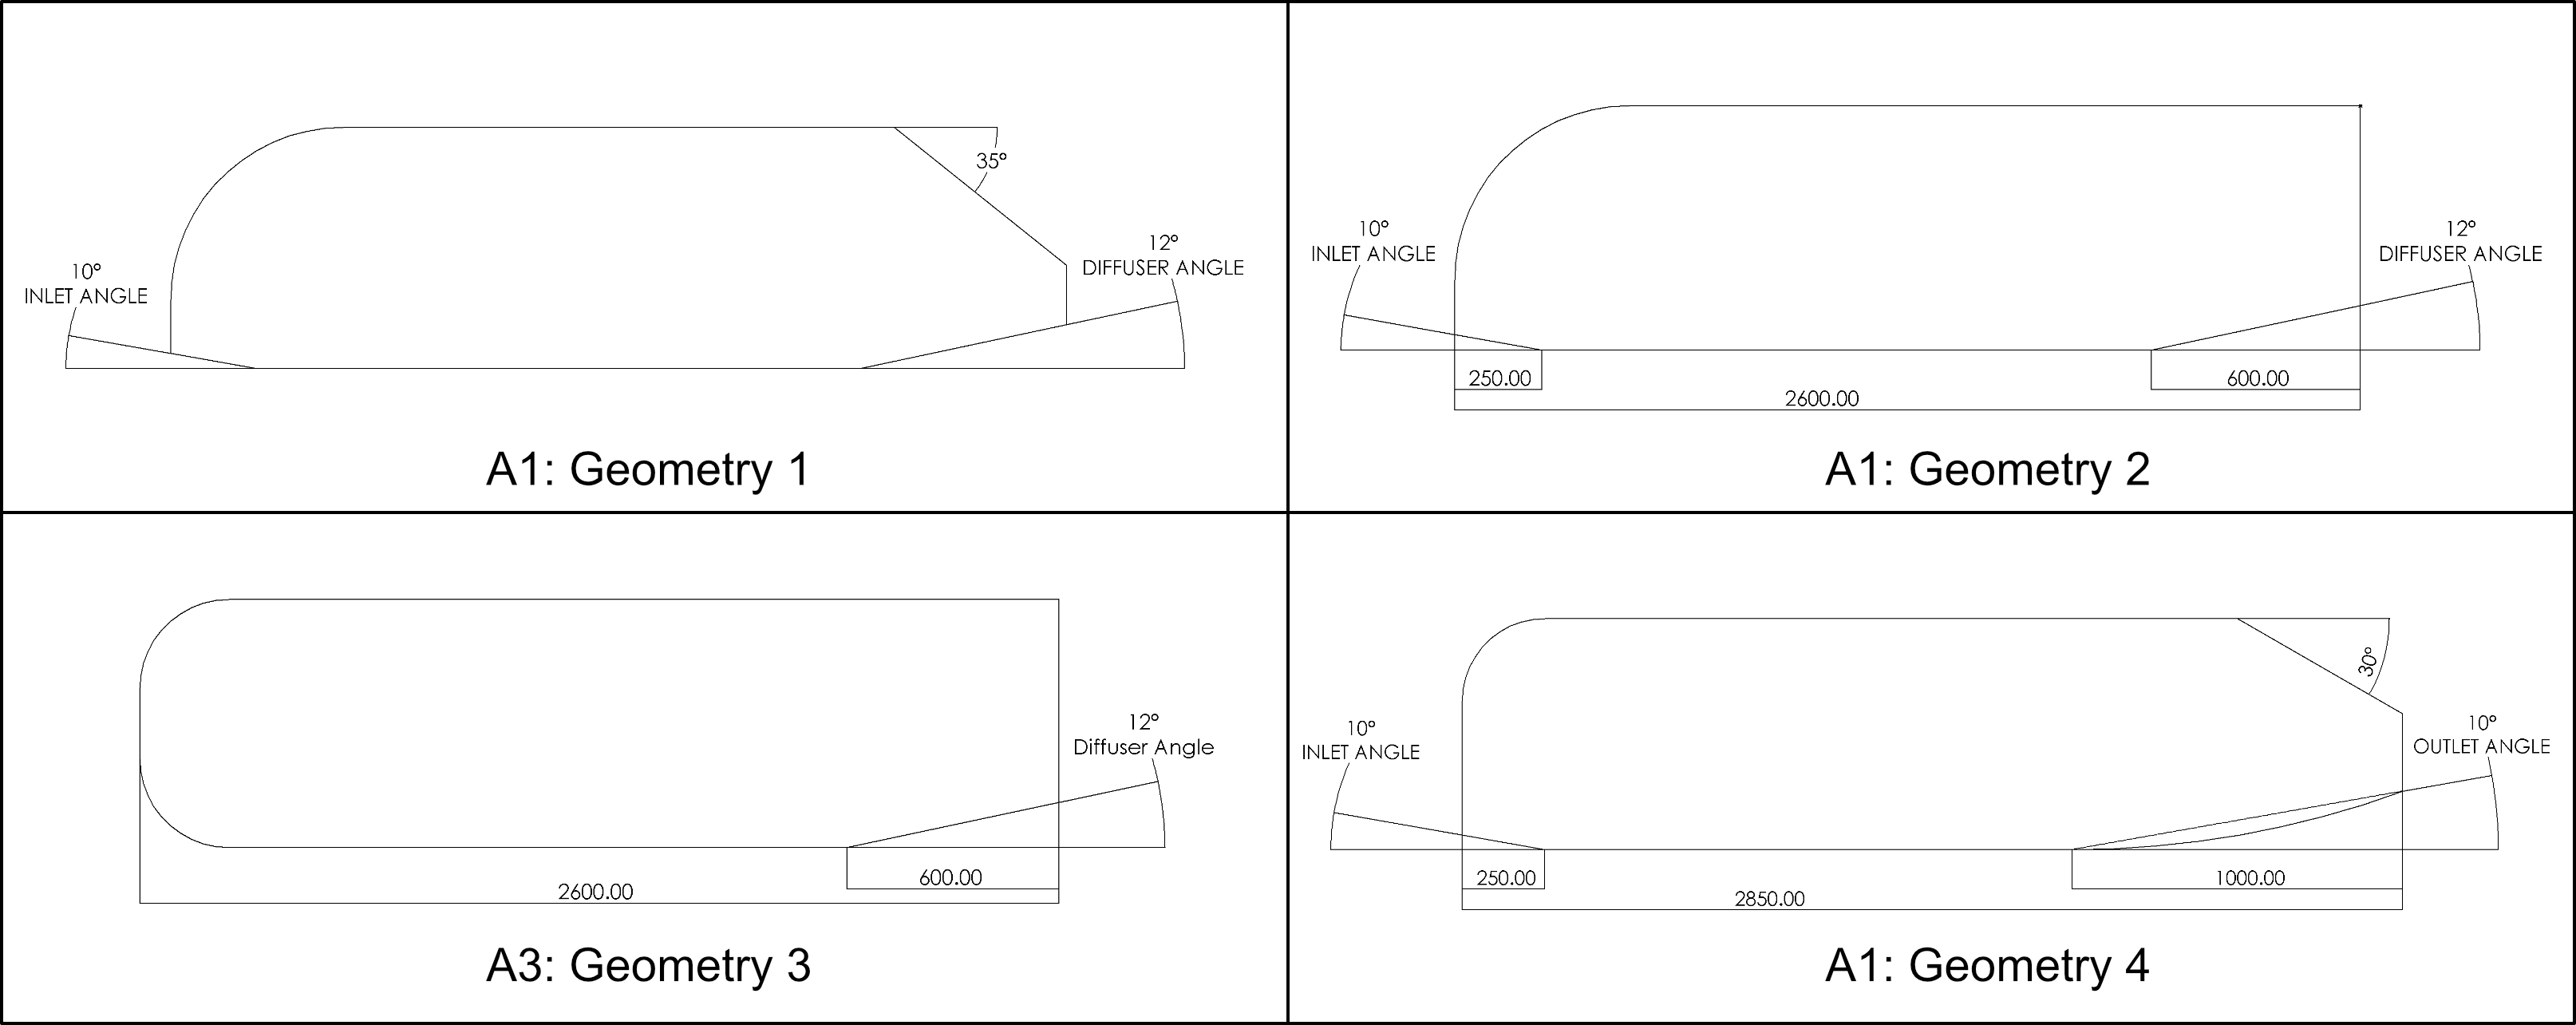
\includegraphics[scale = 0.5]{Figures/2D_OF/2D_OF_GEOM.png}
    \caption{Four Geometries Generated for 2D Open-Flow Analysis.}
    \label{fig:2D_OF_GEOM}
\end{figure}

\noindent The geometries can be grouped into two categories. The first consists of A1 and A2, and focuses on how the geometry of the bluff body sculpts the surrounding flow field and affects the overall performance of the undertray. The first geometry acts as the baseline model, with a 35 degree slant angle at the rear of the body to simulate the kind of flow separation that also occurs at the rear of the QFR car. Geometry 2 has the same dimensions as geometry 1, but without either the inlet angle or the slant angle, to simulate an immediate separation at the rear body.

\noindent The second category consists of geometry 3, which was regenerated as a result of the earlier findings. This geometry used a curved diffuser configuration in which one end was tangential to the throat. A construction line was made between two points of the diffuser as an angle reference point from the horizontal axis. In the diffuser variable angle analysis, a rounded inlet such as geometry 3 without any elevation was used. The purpose of such a rounded intake and diffuser was initially surmised to allow a smooth intake of air and to slow flow separation in the diffuser region by avoiding the sharp transition of the previous geometries. A rear slant angle of 30 degrees was also utilised to provide maximum geometric similarity to the QFR 2021 car.

\noindent A hybrid mesh was generated for this analysis. This consisted of unstructured triangular and quadrilateral elements. An inflation layer was used on the surfaces around the bluff body and the floor to allow the simulation of the effect of the boundary layer interaction between the undertray and floor wall. Detailed graphics of 2D open flow mesh can be seen in Figure~\ref{fig:2D_OF_MESH} in Appendix B.

\subsubsection{Results \& Discussion}

\noindent Two dimensional computational simulations have been carried out, and the results that are shown are based on the downforce and drag of the \textit{entire} bluff body. Analysis 1 and 2 share geometric similarity apart from the slant angle. The first part of the discussion will focus on how the slant angle affects the rear flow and how this impacts on the undertray's performance. Figure~\ref{fig:2D_OF_A12_results} (left) below depicts the trends in downforce and drag with diffuser angle. The variations in lift and drag due to the inlet angle is also shown in Figure~\ref{fig:2D_OF_A12_results} (right).

\begin{figure}[!ht]
    \centering
    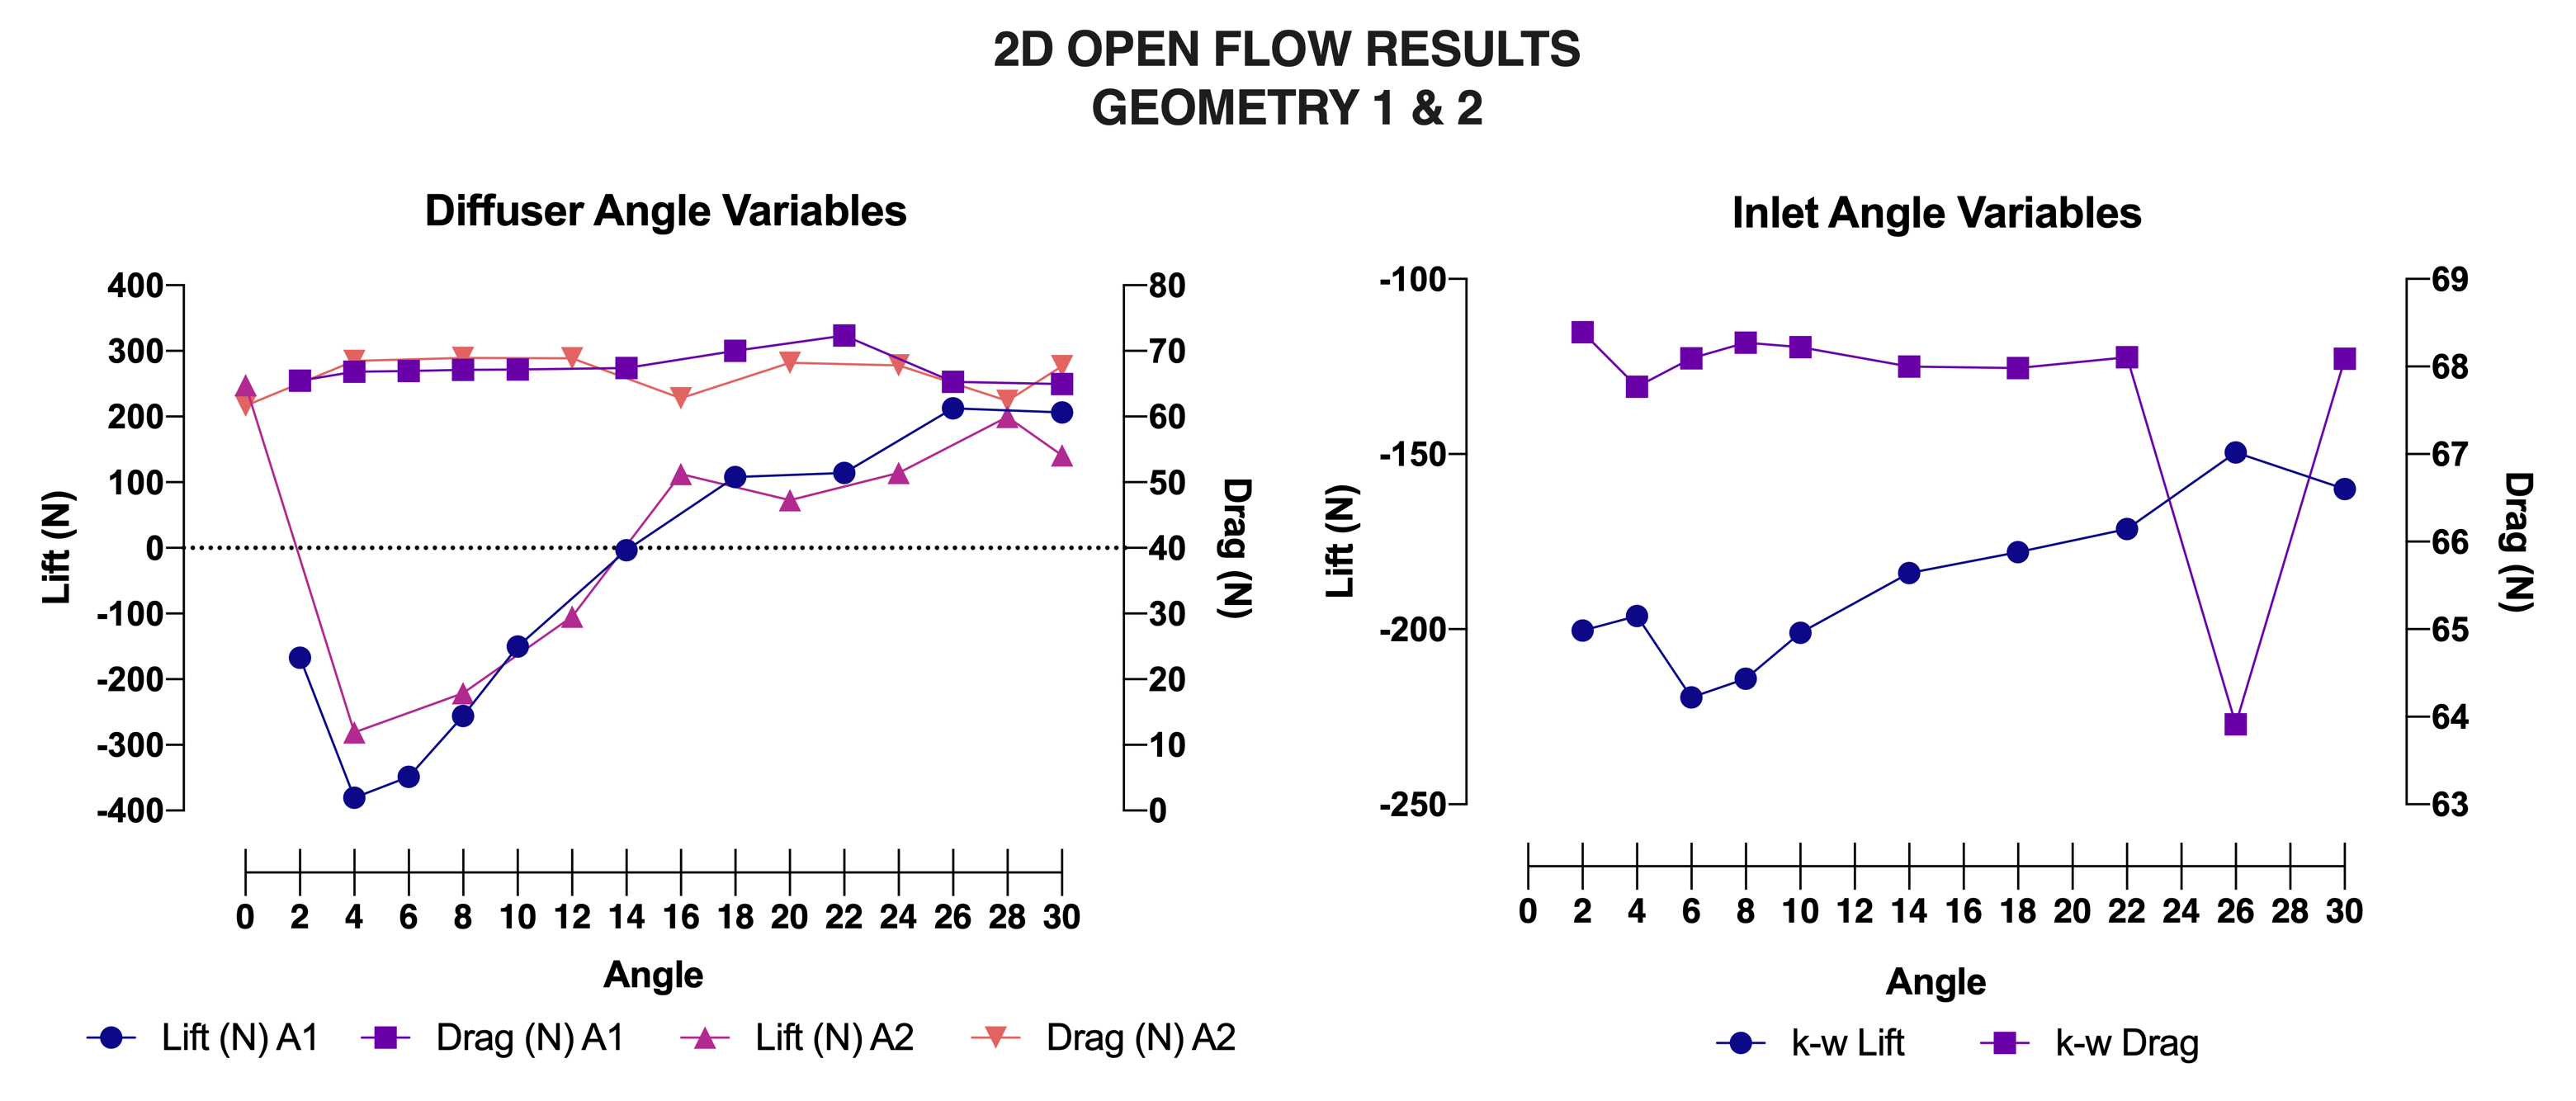
\includegraphics[scale = 0.6]{Figures/Graph/2D_OF_A1-2.png}
    \caption{Lift and Drag Variation vs. Inlet and Diffuser Angle on Geometry 1 and 2.}
    \label{fig:2D_OF_A12_results}
\end{figure}

\noindent The 2D enclosed analysis had a range of 10 to 20 degrees for both inlet and diffuser angles. In Figure~\ref{fig:2D_OF_A12_results} (left), the lift and drag trend due to the diffuser angle elevation can be observed. A significant drop in lift occurred for both A1 and A2 from 0 to 4 degrees. A small angle in the diffuser allows the flow to stay attached all the way to the diffuser wall, allowing for a more gradual increase in pressure that increases the overall downforce. This can be seen on the velocity contour in Figure~\ref{fig:2D_OF_10_4_Contour_compare} (left) below, where the formation of adverse pressure gradient on the diffuser (indicated by the blue region) is delayed at 4 degrees compared to 10 degrees, where separation is occurring around the transition region. Further analysis of the flow separation can be seen in Figure~\ref{fig:2D_OF_10_4_Contour_compare} (right), that shows the comparison of wall shear stress and pressure along the the undertray surface for both geometries 1 and 2. 

\begin{figure}[!htb]
    \centering
    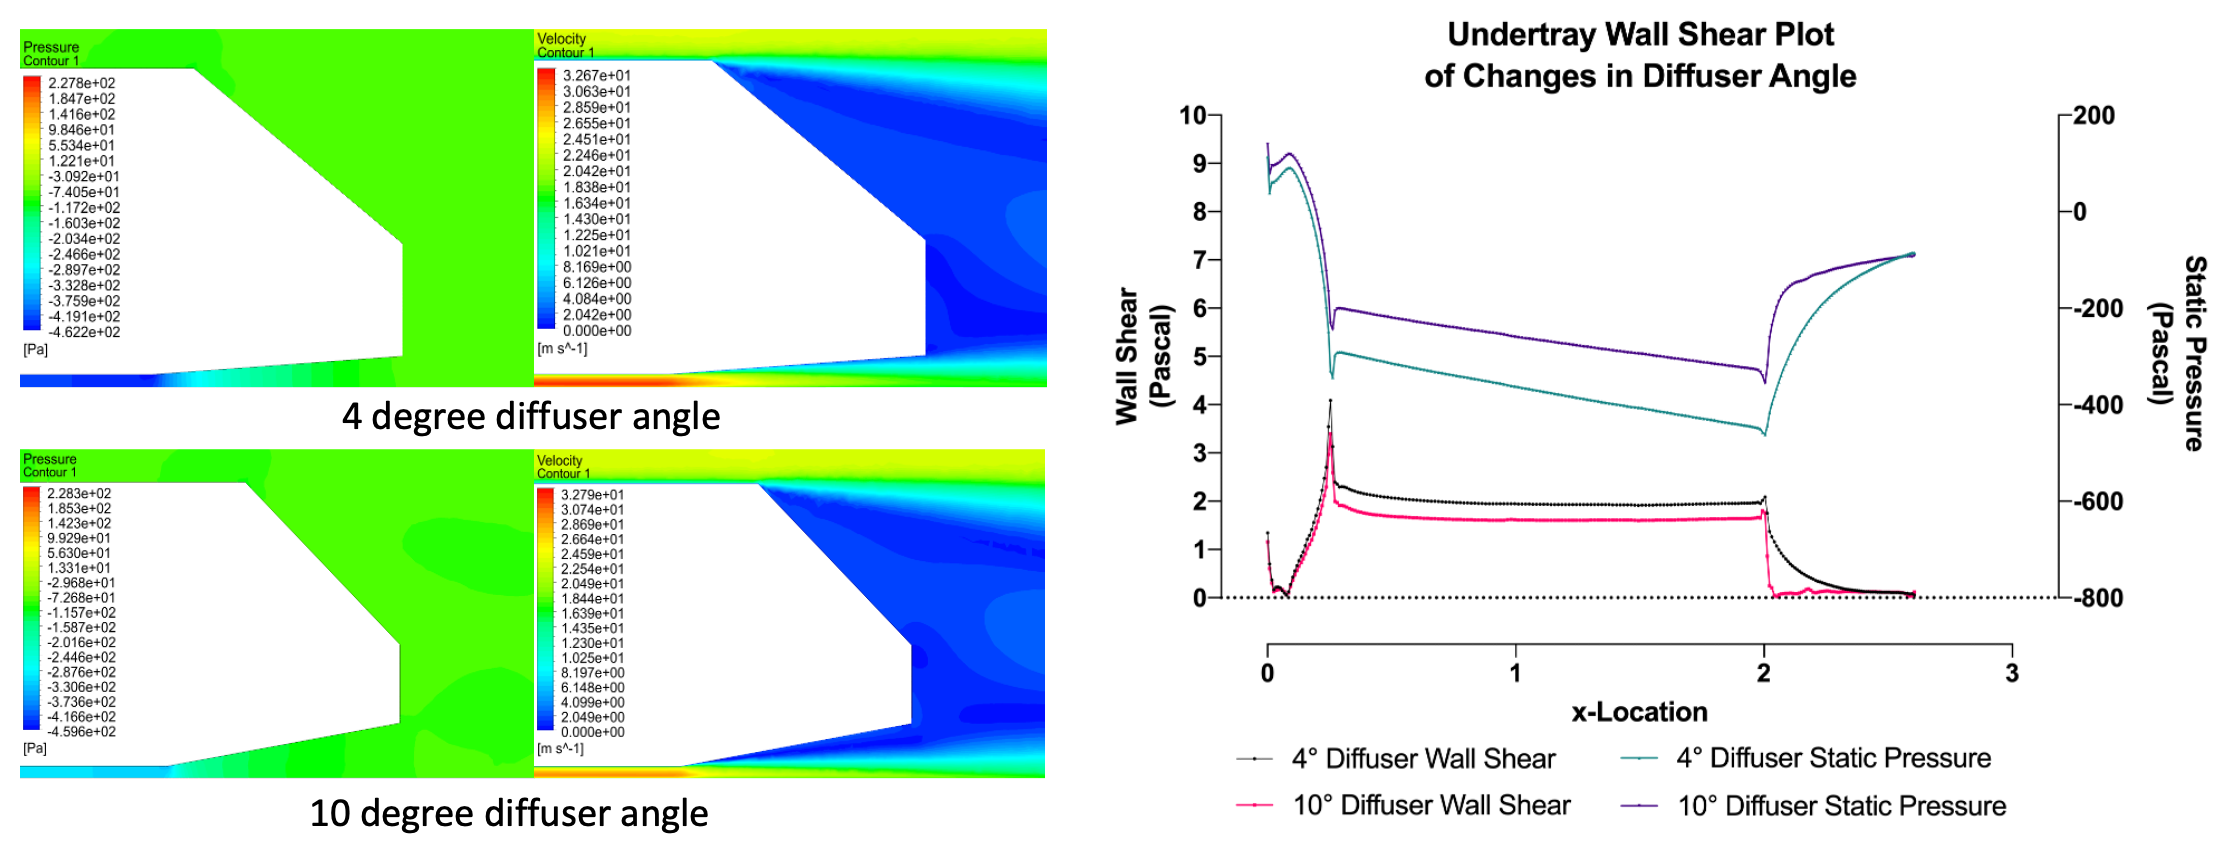
\includegraphics[scale=0.52]{Figures/2D_OF/10_4_O_COMPARE CONTOUR.PNG}
    \caption{Comparison of 4 and 10 Degrees Diffuser Angle With Regard to Flow Separation on the Diffuser Region.}
    \label{fig:2D_OF_10_4_Contour_compare}
\end{figure}

\noindent Following the drop in lift at 4 degrees, a degradation in downforce performance is clear on the graph, following the trend seen in the 2D enclosed lift analysis from 10 to 20 degrees. However, no significant drag changes or trend emerged with the changing of the diffuser angle. From both analyses, the slant angle's presence was deemed to not significantly affect the overall effect on lift and drag of the bluff body on both geometries, which is indicated by an essentially identical lift and drag trend between geometries 1 and 2. It is shown in Figure~\ref{fig:2D_OF_A1_CONTOUR}, in Appendix B, that flow separation occurred immediately at the slant angle, which indicates similar flow features at the rear compared to geometry 2 (Figure~\ref{fig:2D_OF_A2_CONTOUR}, in Appendix B). 

\noindent On the other hand, the inlet variable shows the opposite  trend to that for the 2D enclosed flow, with the inlet angle found to be inversely proportional to the downforce. The flow generates a stagnation point on the front of the bluff body, which acts as the point that separates the oncoming flow into the flow over the body and through the undertray. This slows the velocity of the flow that enters the inlet region, hence reducing the overall effectiveness of the intake. In comparison, the 2D enclosed flow has a perfect flow intake, without any turbulence disturbance or variation in velocity. As it enters the inlet angle of 22 degrees, the low pressure separation region at the intake is insignificant; however, this occurrence is clearer at the transition between the intake and throat, as indicated by the blue velocity streamline highlighted in circle (see fig \ref{fig:A1_Contour_inlet_compare} right). This can be further observed on the inlet pressure plot in Figure~\ref{fig:2D_OF_A1_PLOT} in Appendix B. It can be seen that there is pressure fluctuation for the 6 and 10-degree angles. This indicates the early low-pressure region, as discussed earlier. Moreover, at an inlet elevation of 22 degrees, an immediate pressure drop is indicated on the plot at the transition corner between the inlet and throat region. Moreover, it can be observed that the immediate redirection of the streamlines in Figure~\ref{fig:A1_Contour_inlet_compare} causes a low pressure region.

\begin{figure}[!hb]
   \noindent\makebox[\textwidth]{
   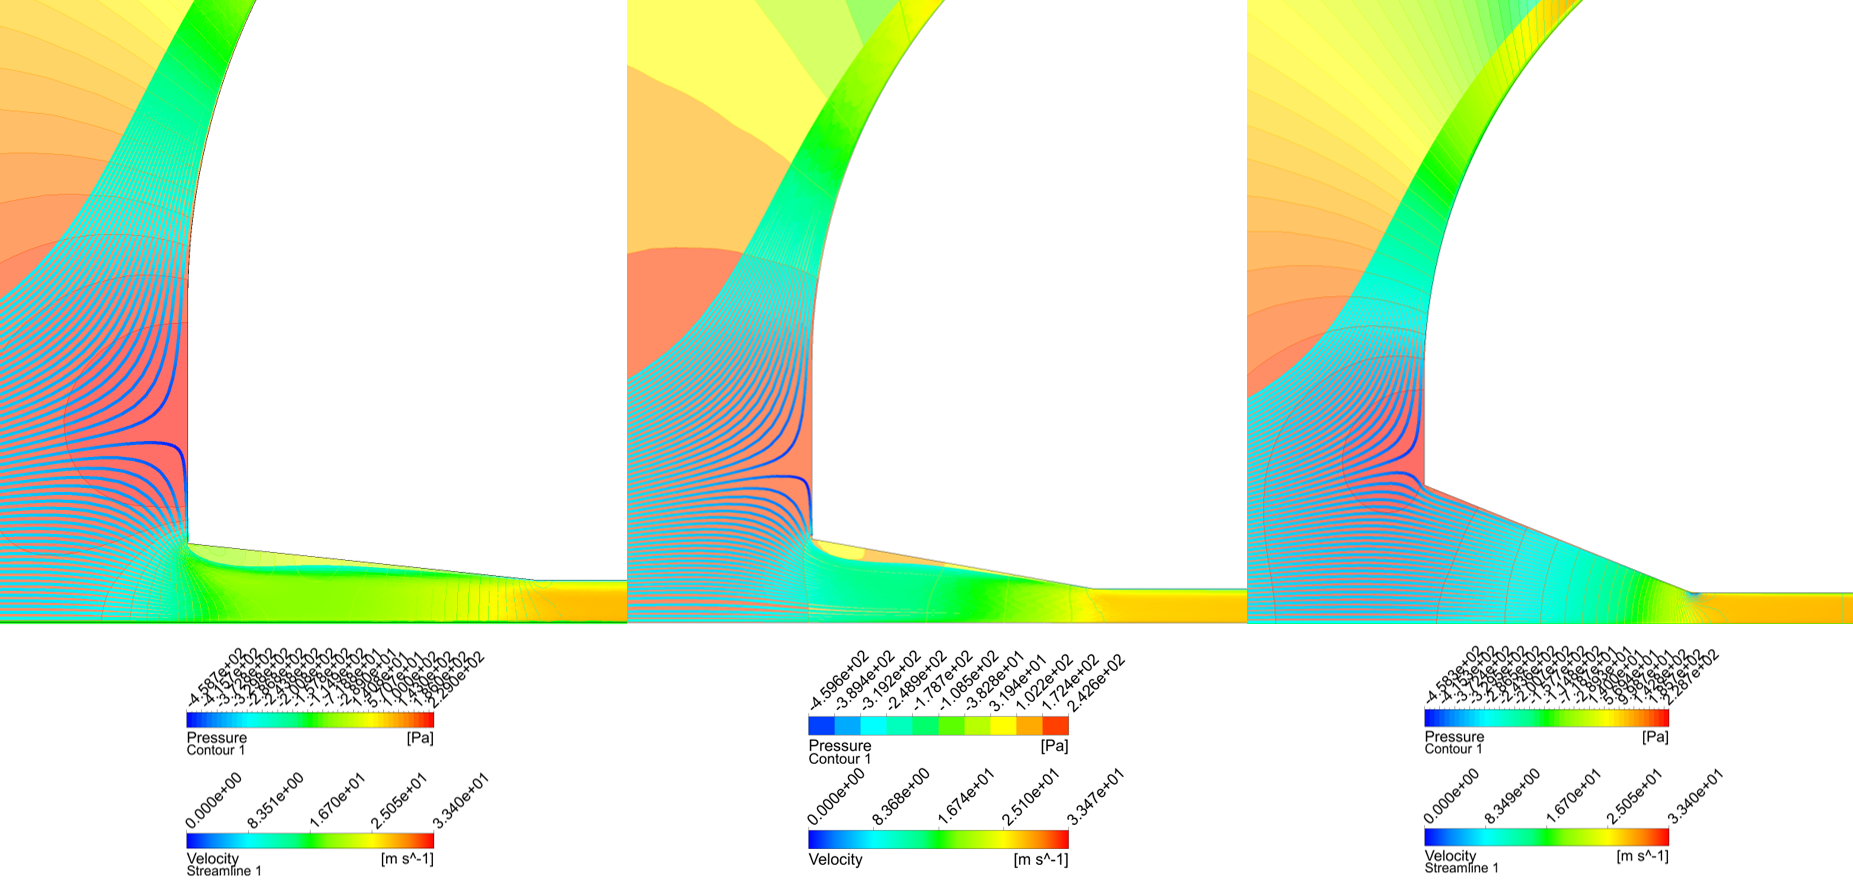
\includegraphics[width=0.8\textwidth]{Figures/2D_OF/2D_OF_A1_CONTOUR_INLET_COMPARE.png}}
   \caption{Comparison of Velocity Streamlines and Pressure Contours for 6 (left), 10 (middle), and 22 (right) Degrees Inlet Angle.}
   \label{fig:A1_Contour_inlet_compare}
\end{figure}

\noindent It was observed that the sharp corner might increase the likelihood of early separation for some geometries. Therefore, geometry 3 was designed to overcome these problems. Figure~\ref{fig:2D_OF_A4_results} below depicts the plot of variation in lift and drag vs inlet and diffuser angle for geometry 3.

\begin{figure}[!ht]
    \noindent\makebox[\textwidth]{
   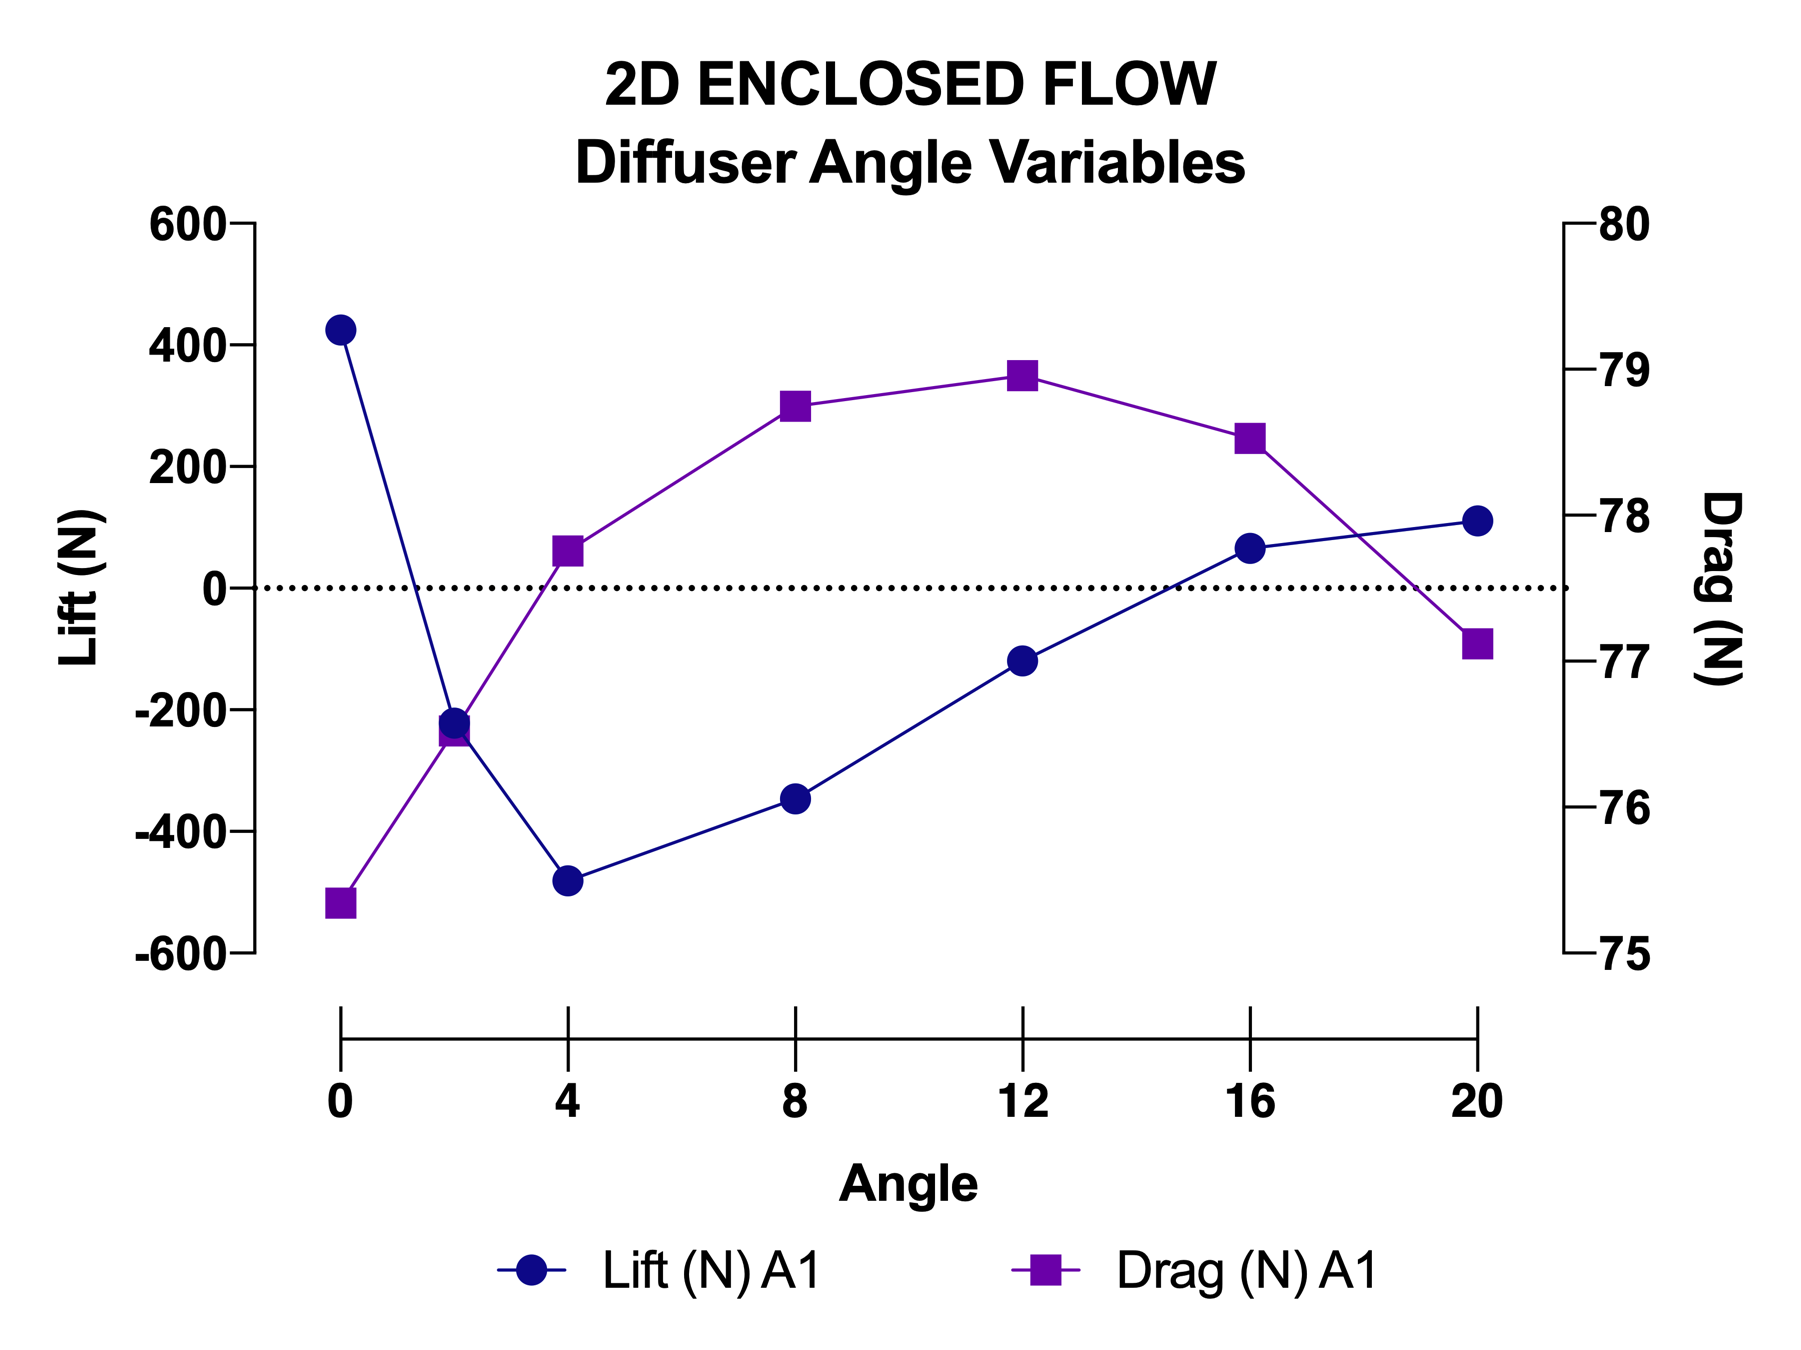
\includegraphics[width=1\textwidth]{Figures/Graph/2D_OF_A3.png}}
    \caption{Lift and Drag Variation vs. Diffuser and Inlet Angle of Geometry 3.}
    \label{fig:2D_OF_A4_results}
\end{figure}

\noindent An identical trend can also be observed for lift vs diffuser angle for both geometries 2 and 3. Maximum downforce was found to occur at a diffuser angle of 5 degrees, which was followed by a linear decrease in downforce. From this analysis alone, flow separation occurs after 5 degrees diffuser angle for both geometry 2 and 3; however, a longer and smoother diffuser has been shown to increase the overall downforce by delaying the separation compared to other geometries. An increase in drag was found to occur up to a maximum at 10 degrees, and then to decrease subsequently; however, it is worth noting that the scale is small, which makes it practically negligible. On the other hand, the inlet variable also shows a similar and clear trend due to the smoother intake. It can be seen that lift smoothly increases proportionally with the inlet angle, which suggests an effective flow intake with no disturbances or flow separation in the inlet region. Comparing the performance of all the geometries analysed, it can be seen from Figure~\ref{fig:2D_OF_PLOT_COMPARE_ALL} below that the overall downforce of geometry 3 at any given angle after 5 degrees is generally lower, and that the overall drag is also generally higher, however insignificantly, compared to the rest of geometries.

\begin{figure}[htb!]
    \centering
    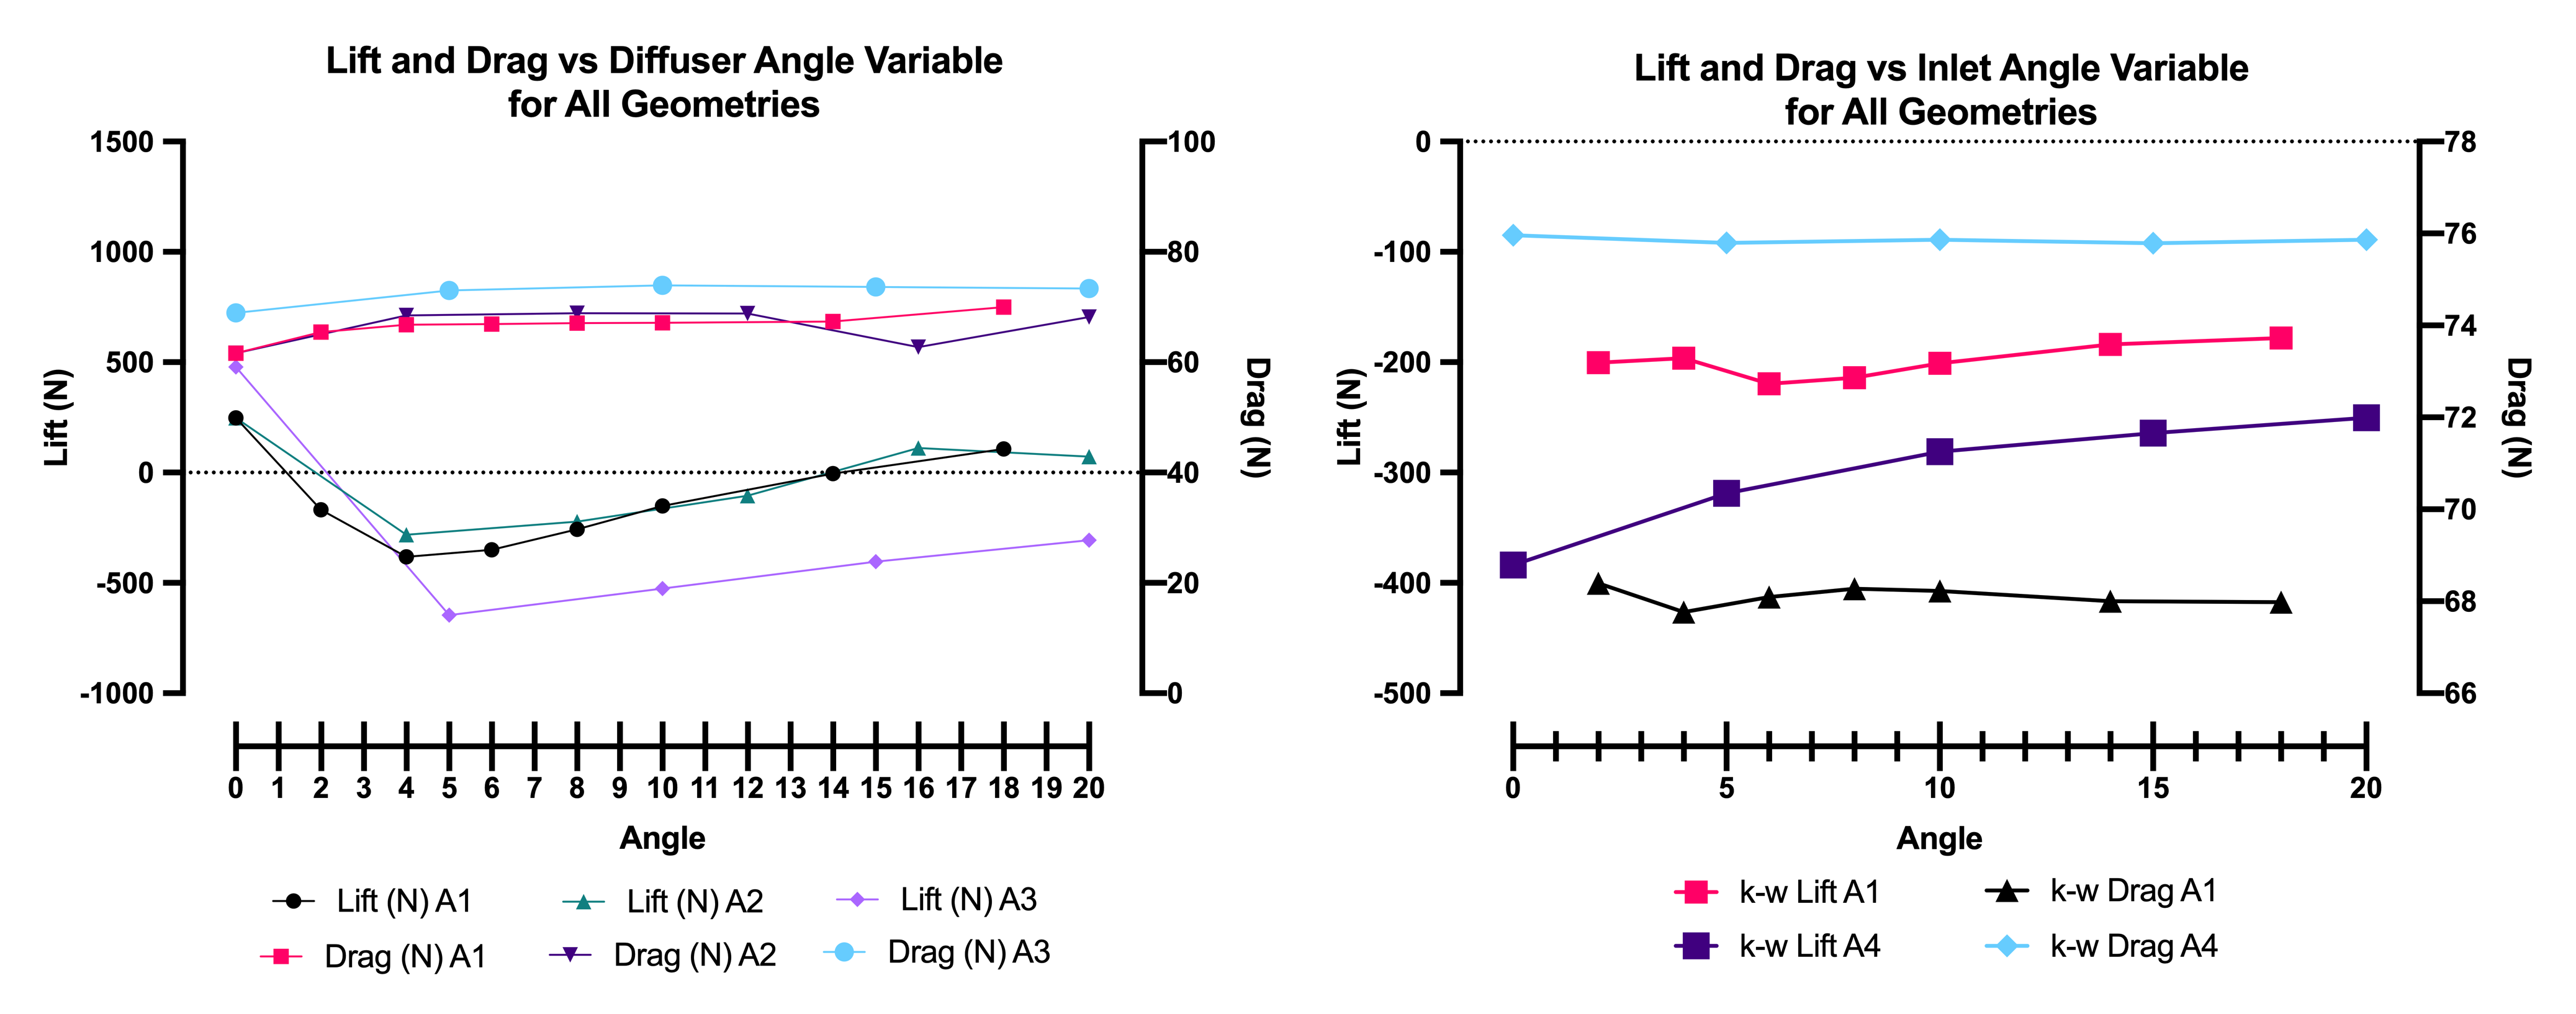
\includegraphics[scale=0.9]{Figures/2D_OF/2D_OF_PLOT_COMPARE_ALL.png}
    \caption{Lift and Drag Variation vs. Diffuser (left) and Inlet (right) Angle of All Geometries.}
    \label{fig:2D_OF_PLOT_COMPARE_ALL}
\end{figure}

\noindent Similarly for the inlet angle variable, a smoothed inlet angle allows for a better flow intake, which is indicated by the overall downforce and drag of geometry 3 being higher than for geometry 1. It is worth noting that the 2D open flow analyses indicate no significant changes in drag for all variables. This is due to the significant drag produced by the flow separation at the rear bluff body itself, unlike in the the 2D enclosed flow, where drag is only produced by the flow underneath. Hence, changes in undertray drag are very small when compared to the bluff body drag.

\noindent A 2D open flow analysis was performed in order to overcome some of the limitations that were observed with the enclosed flow. A body was added above the undertray to help understand the undertray's flow while including the effects of its surroundings, and some different behaviours and new flow physics were observed. However, there were some flow features, such as corner vortices on the diffuser, which this approach was not able to capture, and which  will be resolved in the next section.



